\section{Introduction}
\label{sec:intro}

Supersymmetry (SUSY) is a popular extension to the standard model (SM) of particle physics, which may explain
the 16 orders of magnitude difference between the electroweak and Planck scales (hierarchy problem), introduce
a natural candidate for the dark matter weakly-interacting massive particle (WIMP), and lead to the unification of
gauge couplings.
In order to solve the hierarchy problem without fine-tuning, SUSY must introduce
light top and bottom squarks, the SUSY partners of the top and bottom quarks~\cite{ref:naturalsusy}.
If R-parity is conserved, the lightest SUSY particle (LSP),
usually the lightest neutralino \lsp, is a stable WIMP. If produced in pp collisions this
particle carries away undetected energy and leads to large missing transverse energy (\met).
In this note we present the results of searches for top and bottom squarks in final states with \met, 
using data collected by the Compact Muon Solenoid (CMS)~\cite{ref:CMS} detector at the
Large Hadron Collider (LHC). The data was collected at a center-of-mass energy $\sqrt{s}=8$~TeV in 2012
and corresponds to an integrated luminosity of approximately 10~fb$^{-1}$.

\begin{figure*}
\begin{center}
\subfloat[] {
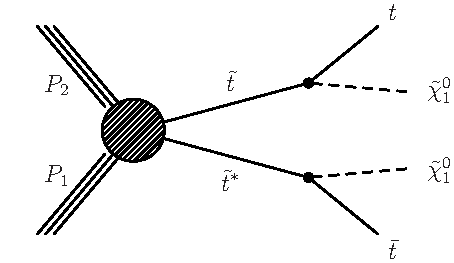
\includegraphics[width=0.35\textwidth]{HCPPlots/T2tt.pdf}
}\quad
\subfloat[] {
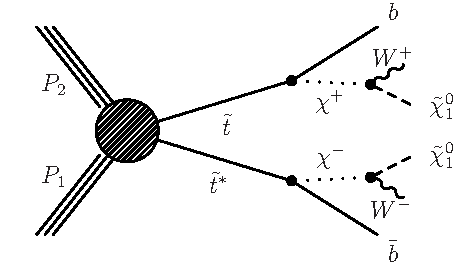
\includegraphics[width=0.35\textwidth]{HCPPlots/T2bw.pdf}
}\quad
\subfloat[] {
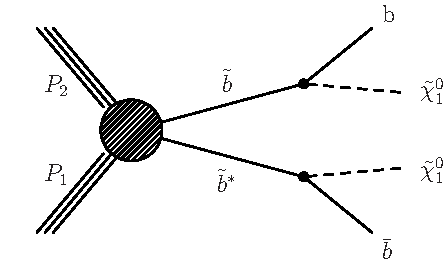
\includegraphics[width=0.35\textwidth]{HCPPlots/T2bb.pdf}
}
\subfloat[] {
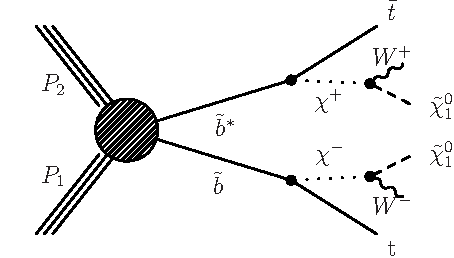
\includegraphics[width=0.35\textwidth]{HCPPlots/T2ttww.pdf}
}
\caption{Example topologies with direct pair production of top (a,b) and bottom (b,c) squarks.
\label{fig:diagrams}
}
\end{center}
\end{figure*}


%\begin{figure*}
%\centering
%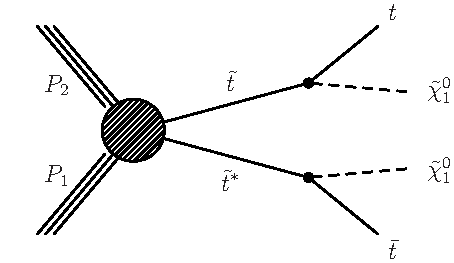
\includegraphics[width=1cm,clip]{HCPPlots/T2tt.pdf}
%% Use the relevant command for your figure-insertion program
%% to insert the figure file. See example above.
%% If not, use
%\vspace*{5cm}       % Give the correct figure height in cm
%\caption{Please write your figure caption here}
%\label{fig:diagrams}       % Give a unique label
%\end{figure*}

Top and bottom squarks may either be produced directly in pairs
(direct pair production) or in the decays of heavier SUSY particles such as the gluino (gluino-mediated squark production). 
In this note we focus on searches for the direct pair production mode.
Examples of such processes are indicated in Fig.~\ref{fig:diagrams}.
The production of these particles may lead to excesses above the SM background expectations in several final states, 
depending on the mass hierarchy of the SUSY particles.
Here we report the results from three searches which focus on the single lepton final state using the transverse
mass~\cite{ref:stop}, the same-sign dilepton final state~\cite{ref:ss}, and the all-hadronic final state~\cite{ref:alphat}.

